%Building
\documentclass[11pt]{article}

\usepackage[english]{babel}
\usepackage[margin=1in]{geometry}
\usepackage[colorlinks=true, allcolors=blue]{hyperref}

% Math/Greek packages
\usepackage{amssymb, amsmath, amsthm, mathtools, esint} 
\usepackage{algorithm, algorithmic}
\usepackage{upgreek}
\usepackage{physics}

% Graphics/Presentation packages
\usepackage{graphicx}
\usepackage{multirow, subcaption, cleveref}
\usepackage{tabulary, enumitem}
\usepackage{cancel}

%replace "ref" with "cref", "Cref", "crefrange"

% Misc packages
\renewcommand\qedsymbol{\textit{``Quack"}} %change the QED symbol to ``Quack" for the inside joke of Quantum Entangled Ducks

% defining where the images are
\graphicspath{ {../ESOF 322 Project (drive copy)/} }


%\usepackage{fontspec}
% Use this line to change the font of your file. If you have the Open Dyslexic v. 1 downloaded (bold-italic- bolditalics included) you can use this line. This font addresses Dyslexic peoples. 
%\setmainfont{OpenDyslexic}
% Use this line to change the font of your file. If you have the Atkinson Hyperlegible downloaded (bold-italic- bolditalics included) you can use this line. This font addresses sight-impared peoples
% \setmainfont{Atkinson Hyperlegible}

\begin{document}

\title{ESOF 322: Project 1 - Cold Case Database}
\author{Jacob Coleman, William Jardee, Fletcher Philips, Megan Steinmasel}
\maketitle


%%TO-DO
% check for any implementation in usecases

\textbf{System Description}: In the world of criminal justice, it is not a rare occurrence that the truth is thinly veiled by a lack of gathered evidence or proper techniques to analyze current data. A prime example of this is the aid of DNA testing in prosecution. The proposed software system will collect old and new evidence into one database (centralized storage system), organize it, and present it to domain specialists through an easy-to-use website. The initial construction of this project is humble but aims to create a skeleton for more sophisticated analysis techniques to be built on. It is assumed that there are two primary ways to interact with the system: through control of the database operations and in the form of the website; these are the database engineer and website user, respectively.\vspace{1.5em}

\textit{Database Engineer}: An individual knowledgeable of how the system works and responsible for maintenance and updates.\vspace{0.5em}

\textit{Website  User}: A front-end user that likely lacks data science knowledge traversing the web system.\vspace{0.5em}

\textit{Criminal Justice Professional}: Someone in the field of criminal justice who will be using our system to make their job easier (This is synonymous with Website User).\vspace{0.5em}

\vspace{1em}


\section*{User Stories}

\noindent\textbf{Epic}: As a Criminal Justice Professional, I want a database that can hold, sort, and present data according to a variety of different queries and eventually use state-of-the-art algorithms to help me succeed in my job.\vspace{0.5em}

\noindent\textbf{\hypertarget{us1}{User Story 1}} (Megan Steinmasel):  As a website User, I want a search bar that will search the database.\vspace{0.5em}

\noindent\textbf{\hypertarget{us2}{User Story 2}} (William Jardee): As a website user, I need the processing of data to be done automatically in a way that is friendly to someone that is not a data scientist.\vspace{0.5em}

\noindent\textbf{\hypertarget{us3}{User Story 3}} (Jacob Coleman): As a website user, I want a data visualization technique that is intuitive and accurately shows patterns in the data.\vspace{0.5em}

\noindent\textbf{\hypertarget{us4}{User Story 4}} (Fletcher Philips): As a database engineer, I want to have a database so that I can store cold cases inside of it. \vspace{0.5em}

\noindent\textbf{\hypertarget{us5}{User Story 5}} (Fletcher Philips): As a database engineer, I want a central storage system so that the admin can insert and delete data.\vspace{0.5em}

\clearpage
%-----------------------------------------------------------------------------------------
%-----------------------------------------------------------------------------------------



\section*{UseCase Diagram}

\begin{figure}[!ht]
\centering
\textbf{Author: William Jardee}\\
\textit{It should be noted that while William created this iteration of a UseCase Diagram, it is the combination of numerous individual diagrams made by each member of the group.}\vspace{0.5em}

	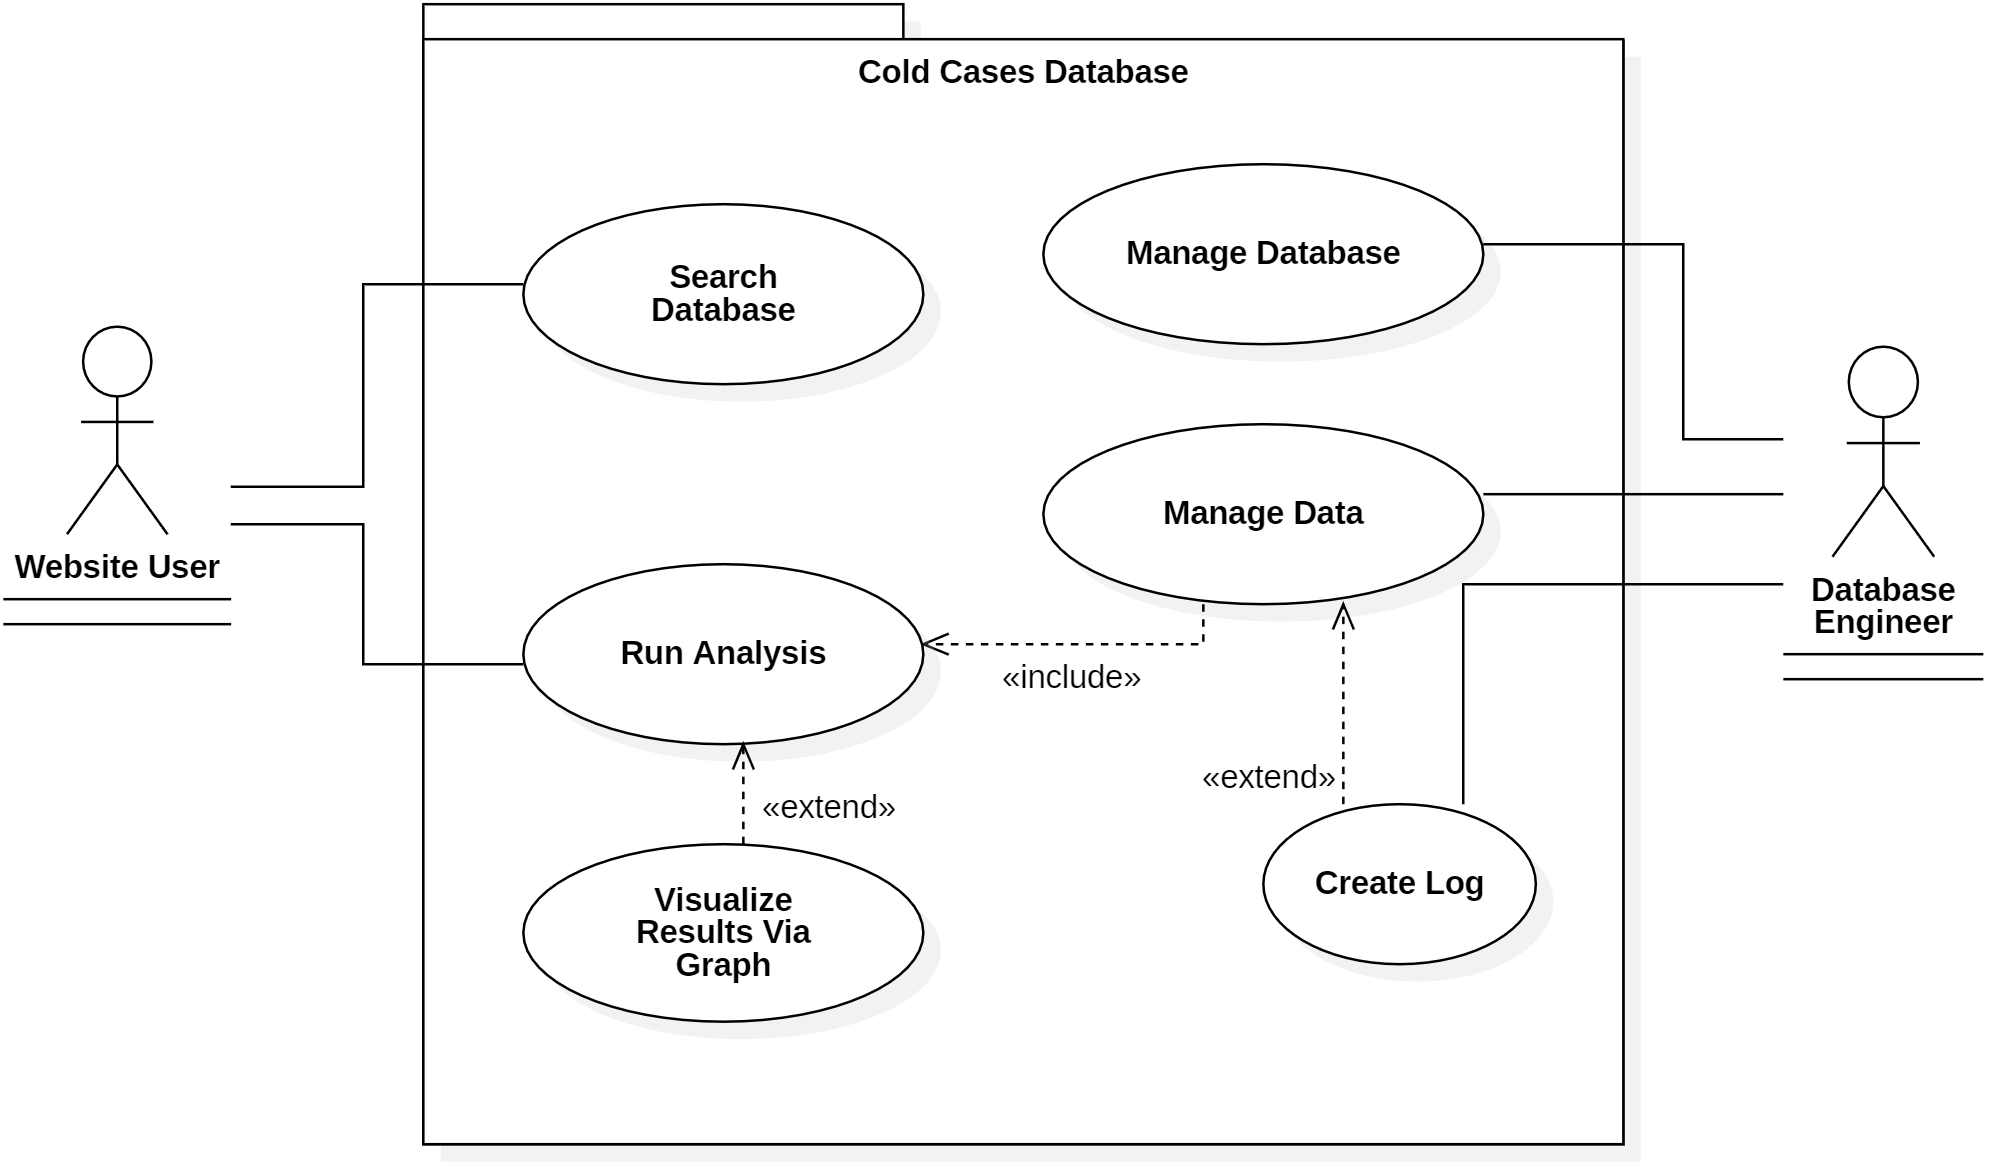
\includegraphics[width=.95\textwidth]{./UseCases/jardee_usecase_3}\\
	\caption{UseCase Diagram for the Cold-Cases Database system.}
	\label{fig:usecase_diagram}
\end{figure}
\clearpage



\subsection*{Textual Descriptions}

%------------------------------------
%Search - Navigation Menu
%------------------------------------
\begin{table}[!ht]
\begin{center}
\textbf{Author: Megan Steinmasel}
\vspace*{1em}

\begin{tabular}{p{0.30\linewidth}p{0.60\linewidth}}
	Name: & Search Database\\\hline
	Description: & Search bar scans keywords through the database so that the Website User can find a desired query/page.\\\hline
	Related Requirements:& \hyperlink{us1}{User Story 1}\\\hline
	Preconditions:& The user has successfully logged onto the website.\\\hline
	Successful end condition:& Successful display of search bar and successful redirection.\\\hline
	Failed end condition:& Search bar is not displayed or failed redirection. \\\hline
	Actors:& Website User\\\hline
	Basic Flow of Events: & \begin{enumerate}
	\item Actor types in keywords to the search bar and clicks enter or selects a page to navigate to.
	\item Request is processed and database is searched.
	\item The appropriate query/page is displayed.
	\end{enumerate}\\\hline
	Extensions/Exceptional Flow of Events: & \begin{enumerate}
	\item An error is recognized: search bar is not displayed and/or failed redirection.
	\item Actor is notified of an error.
	\item Log data.
	\item The Actor is prompted for a refresh of the webpage.
	\item When refresh button is pressed, system reboots and tries again.
	\end{enumerate}
\end{tabular}
\label{des:search_nav_menu}	
\end{center}
\end{table}
%------------------------------------


%------------------------------------
%Create Database
%------------------------------------
\begin{table}[!ht]
\begin{center}
\textbf{Author: Fletcher Philips}
\vspace*{1em}

\begin{tabular}{p{0.30\linewidth}p{0.60\linewidth}}
	Name: & Manage Database\\\hline
	Description: & The database that contains all the data will be maintained. This included initial creation, implementation of new features, and regular maintenance.\\\hline
	Related Requirements:& \hyperlink{us4}{User Story 4}\\\hline
	Preconditions:& Basic web infrastructure has been created. A small sample set of cold cases is ready to be inserted. The current actor has the proper credentials.\\\hline
	Successful end condition:& The database is able to be manipulated in the desired manner.\\\hline
	Failed end condition:& Requested changed cannot be done.\\\hline
	Actors:& Database Engineer\\\hline
	Basic Flow of Events: & \begin{enumerate}
	%THIS IS TOO TECHNICAL
	\item The current state of the database is displayed.
	\item A new change or maintenance is done to the system and attempted to be launched.
	\item The new state of the system is valid and becomes live.
	\end{enumerate}\\\hline
	Extensions/Exceptional Flow of Events: & \begin{enumerate}
	\item Database fails to build properly.
	\item The engineer is notified that an error has appeared.
	\item Log data.
	\item Engineer is returned to the state before the change was added.
	\end{enumerate}
\end{tabular}
\label{des:create_database}	
\end{center}
\end{table}
%------------------------------------

%------------------------------------
%Manage Data
%------------------------------------
\begin{table}[!ht]
\begin{center}
\textbf{Author: William Jardee}
\vspace*{1em}

\begin{tabular}{p{0.30\linewidth}p{0.60\linewidth}}
	Name: & Manage Data\\\hline
	Description: & Data needs to be inserted, deleted, and manipulated. Related to this, there must be an appropriate interface to do this through. The data will connect directly with the database.\\\hline
	Related Requirements:& \hyperlink{us2}{User Story 2}, \hyperlink{us5}{User Story 5}\\\hline
	Preconditions:& The user is logged on and has gained access rights according to their credentials.\\\hline
	Successful end condition:& Data is successfully manipulated, and a success message is received from the source. \\\hline
	Failed end condition:& Requested task is outside of credentials. Success message not received. Invalid new data.\\\hline
	Actors:& Database Engineer\\\hline
	Basic Flow of Events: & \begin{enumerate}
	\item Actor selects the action they wish to do and what to do it on.
	\item Change is enacted.
	\item Flow is complete and prompts the user for the next action.
	\end{enumerate}\\\hline
	Extensions/Exceptional Flow of Events: & \begin{enumerate}
	\item Conflict happens.
	\item Reject any attempted changes and revert any changes.
	\item Notify the actor that there has been an error and log data.
	\item Flow is complete and prompts the user for the next action.
	\end{enumerate}
\end{tabular}
\label{des:man_dat}	
\end{center}
\end{table}
%------------------------------------


%------------------------------------
%Run Analysis
%------------------------------------
\begin{table}[!ht]
\begin{center}
\textbf{Author: William Jardee}
\vspace*{1em}

\begin{tabular}{p{0.30\linewidth}p{0.60\linewidth}}
	Name: & Run Analysis\\\hline
	Description: & An understandable interface for viewing data and selecting data visualization.\\\hline
	Related Requirements:& \hyperlink{us2}{User Story 2}, \hyperlink{us3}{User Story 3}\\\hline
	Preconditions:& The website user has signed into the website and accessed the drop-down menu to access the page. \\\hline
	Successful end condition:& A valid group of data is selected, a visualization format is selected, and the servers are available for the request.\\\hline
	Failed end condition:& One of the above three requirements has been violated, and the window is closed.\\\hline
	Actors:& Website User\\\hline
	Basic Flow of Events: & \begin{enumerate}
	\item A query selection screen is presented, and the desired data is collected.
	\item The type of visualization is selected from a dropdown menu.
	%Do we remove "Via graph?"
	\item The request is sent to the ``Visualize Results via Graph" action.
	\end{enumerate}\\\hline
	Extensions/Exceptional Flow of Events: & \begin{enumerate}
	\item One of the system-side error states was reached.
	\item Report the error to the actor.
	\item Log data.
	\item Return actor back to the homepage.
	\end{enumerate}
\end{tabular}
\label{des:run_anal}	
\end{center}
\end{table}
%------------------------------------


%------------------------------------
%Visualize Results via Graphs
%------------------------------------
\begin{table}[!ht]
\begin{center}
\textbf{Author: Jacob Coleman}
\vspace*{1em}

\begin{tabular}{p{0.30\linewidth}p{0.60\linewidth}}
	Name: & Visualize Results via Graph\\\hline
	Description: & Displays selected graphs from the gathered data\\\hline
	Related Requirements:& \hyperlink{us3}{User Story 3}\\\hline
	Preconditions:& The website user has signed into the website and accessed the page. Some data has been selected for analysis, and the desired type of graph has been selected.\\\hline
	Successful end condition:& The graphs are displayed on a separate page to view.\\\hline
	Failed end condition:& Fails to display any graphs.\\\hline
	Actors:& Website User\\\hline
	Basic Flow of Events: & 
	\begin{enumerate}
	\item The website user goes through a data selection process.
	\item The website user goes through a visualization selection menu.
	\item The system will display any applicable graphics.
	\end{enumerate}\\\hline
	Extensions/Exceptional Flow of Events: & 
	\begin{enumerate}
	\item The graphics fail to display.
	\item The User is notified that the user cannot access graphics.
	\item Log data.
	\item User is sent back to the homepage.
	\end{enumerate}
\end{tabular}
\label{des:vis_res}	
\end{center}
\end{table}
%------------------------------------


%------------------------------------
%Creaete Log
%------------------------------------
\begin{table}[!ht]
\begin{center}
\textbf{Author: William Jardee}
\vspace*{1em}

\begin{tabular}{p{0.30\linewidth}p{0.60\linewidth}}
	Name: & Create Log\\\hline
	Description: & A log file should be kept to track flow and diagnose errors and suspicious behavior.\\\hline
	Related Requirements:& Catch all location for all errors (no specific user story)\\\hline
	Preconditions:& The system has been started effectively, and there is a safe place to store a text file (log file).\\\hline
	Successful end condition:& Data can be saved to the log file.\\\hline
	Failed end condition:& Data cannot be safely saved to a log file.\\\hline
	Actors:& Database Engineer \\\hline
	Basic Flow of Events: & 
	\begin{enumerate}
	\item Write to file recent activity.
	\item Flag any invalid actions prompt ``Log data."
	\end{enumerate}\\\hline
	Extensions/Exceptional Flow of Events: & 
	\begin{enumerate}
	\item Notify the system admin of the issue and include error information.
	\item Terminate all systems until the issue is resolved.
	\end{enumerate}
\end{tabular}
\label{des:create_log}
\end{center}
\end{table}
%------------------------------------

\clearpage
%-----------------------------------------------------------------------------------------
%-----------------------------------------------------------------------------------------



\section*{Class Diagram}

\begin{figure}[!ht]
\centering
\textbf{Author: Fletcher Philips}
	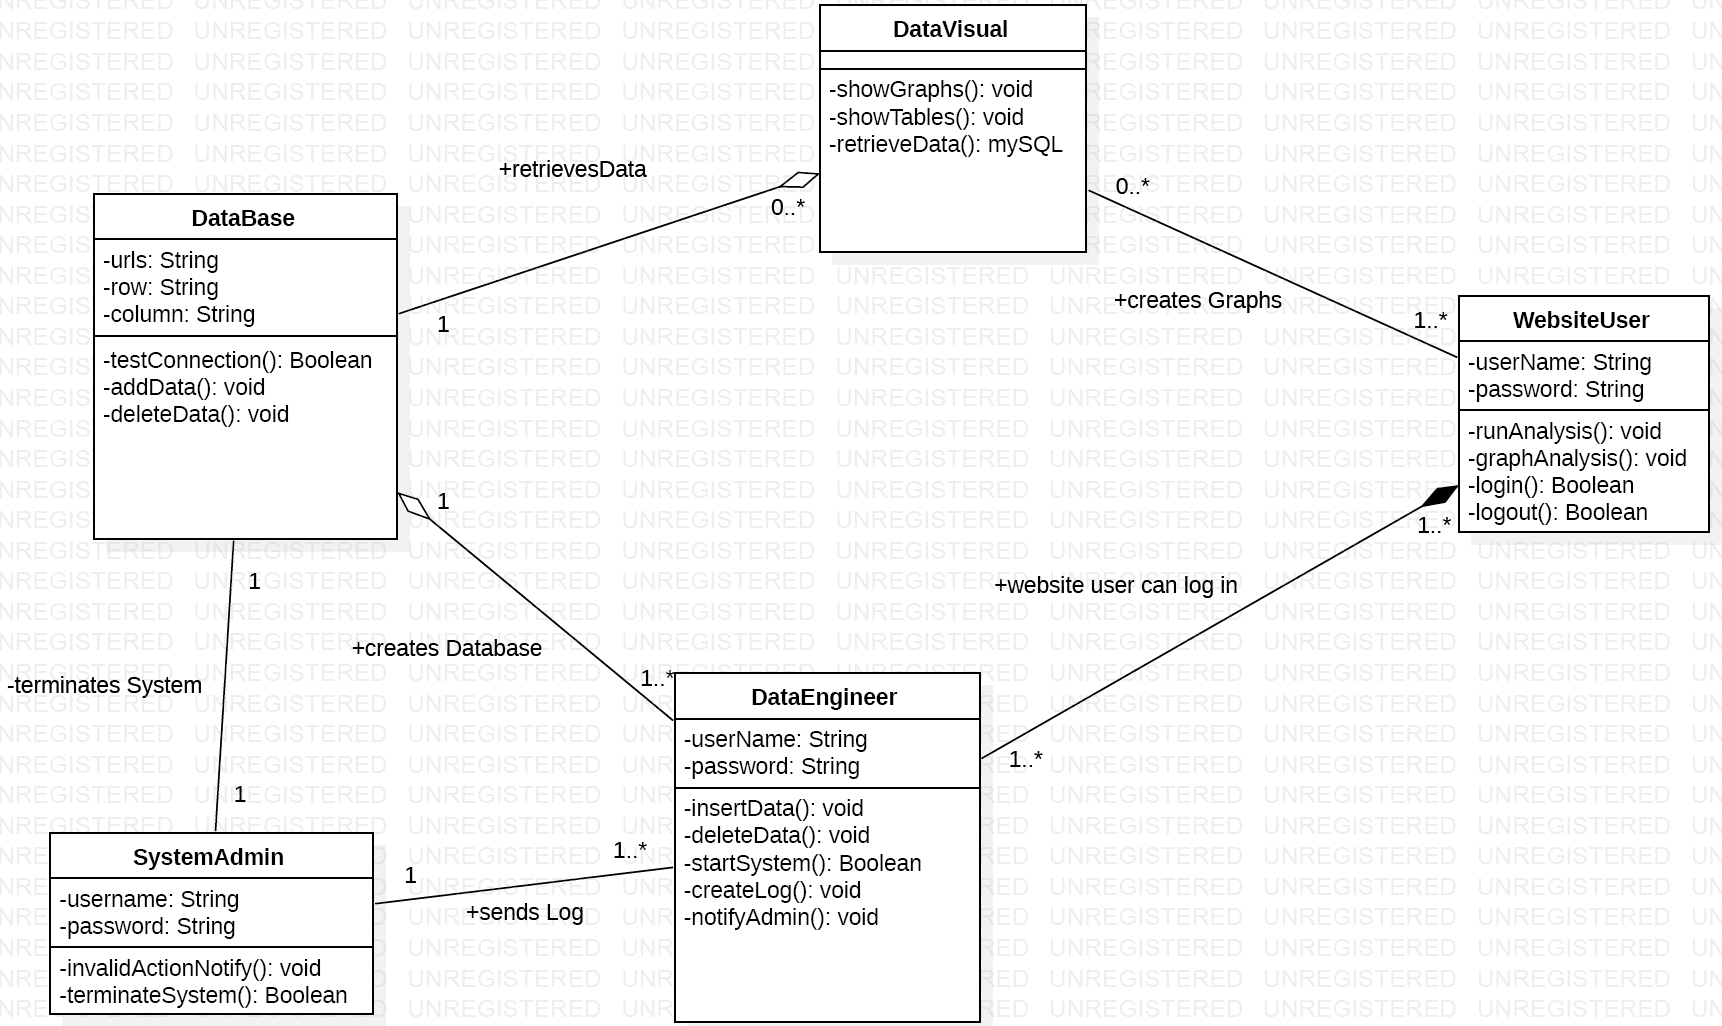
\includegraphics[width=0.9\textwidth]{./Class Diagrams/ColdCaseClassDiagram.png}\\
	\caption{Class Diagram for the Cold-Cases Database system.}
	\label{fig:class_diagram}
\end{figure}
\clearpage
%-----------------------------------------------------------------------------------------
%-----------------------------------------------------------------------------------------



\section*{State Chart Diagram}

\begin{figure}[!ht]
\centering
\textbf{Author: Megan Steinmasel}
	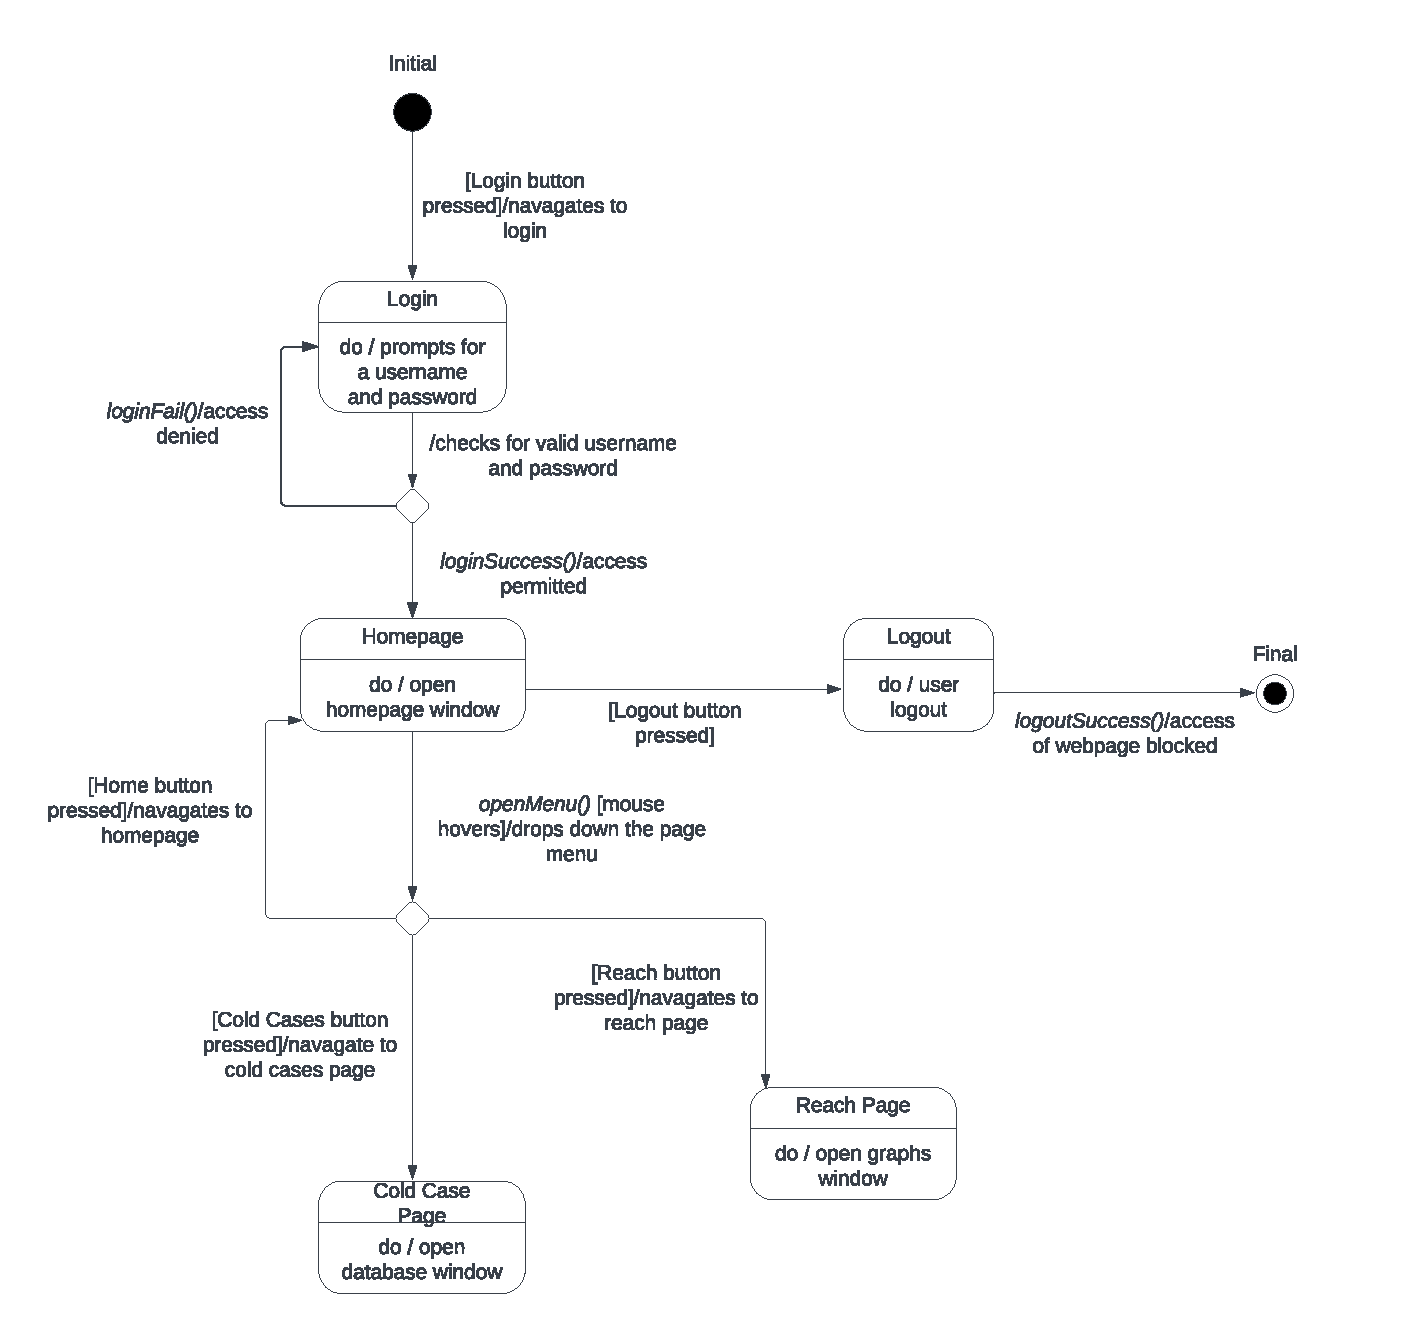
\includegraphics[width=.95\textwidth]{./State Chart/C.C. Statechart}\\
	\caption{State Chart Diagram for the Cold-Cases Database system.}
	\label{fig:state_chart_diagram}
\end{figure}
\clearpage
%-----------------------------------------------------------------------------------------
%-----------------------------------------------------------------------------------------



\section*{Activity Diagram}

\begin{figure}[!ht]
\centering
\textbf{Author: Jacob Coleman}
	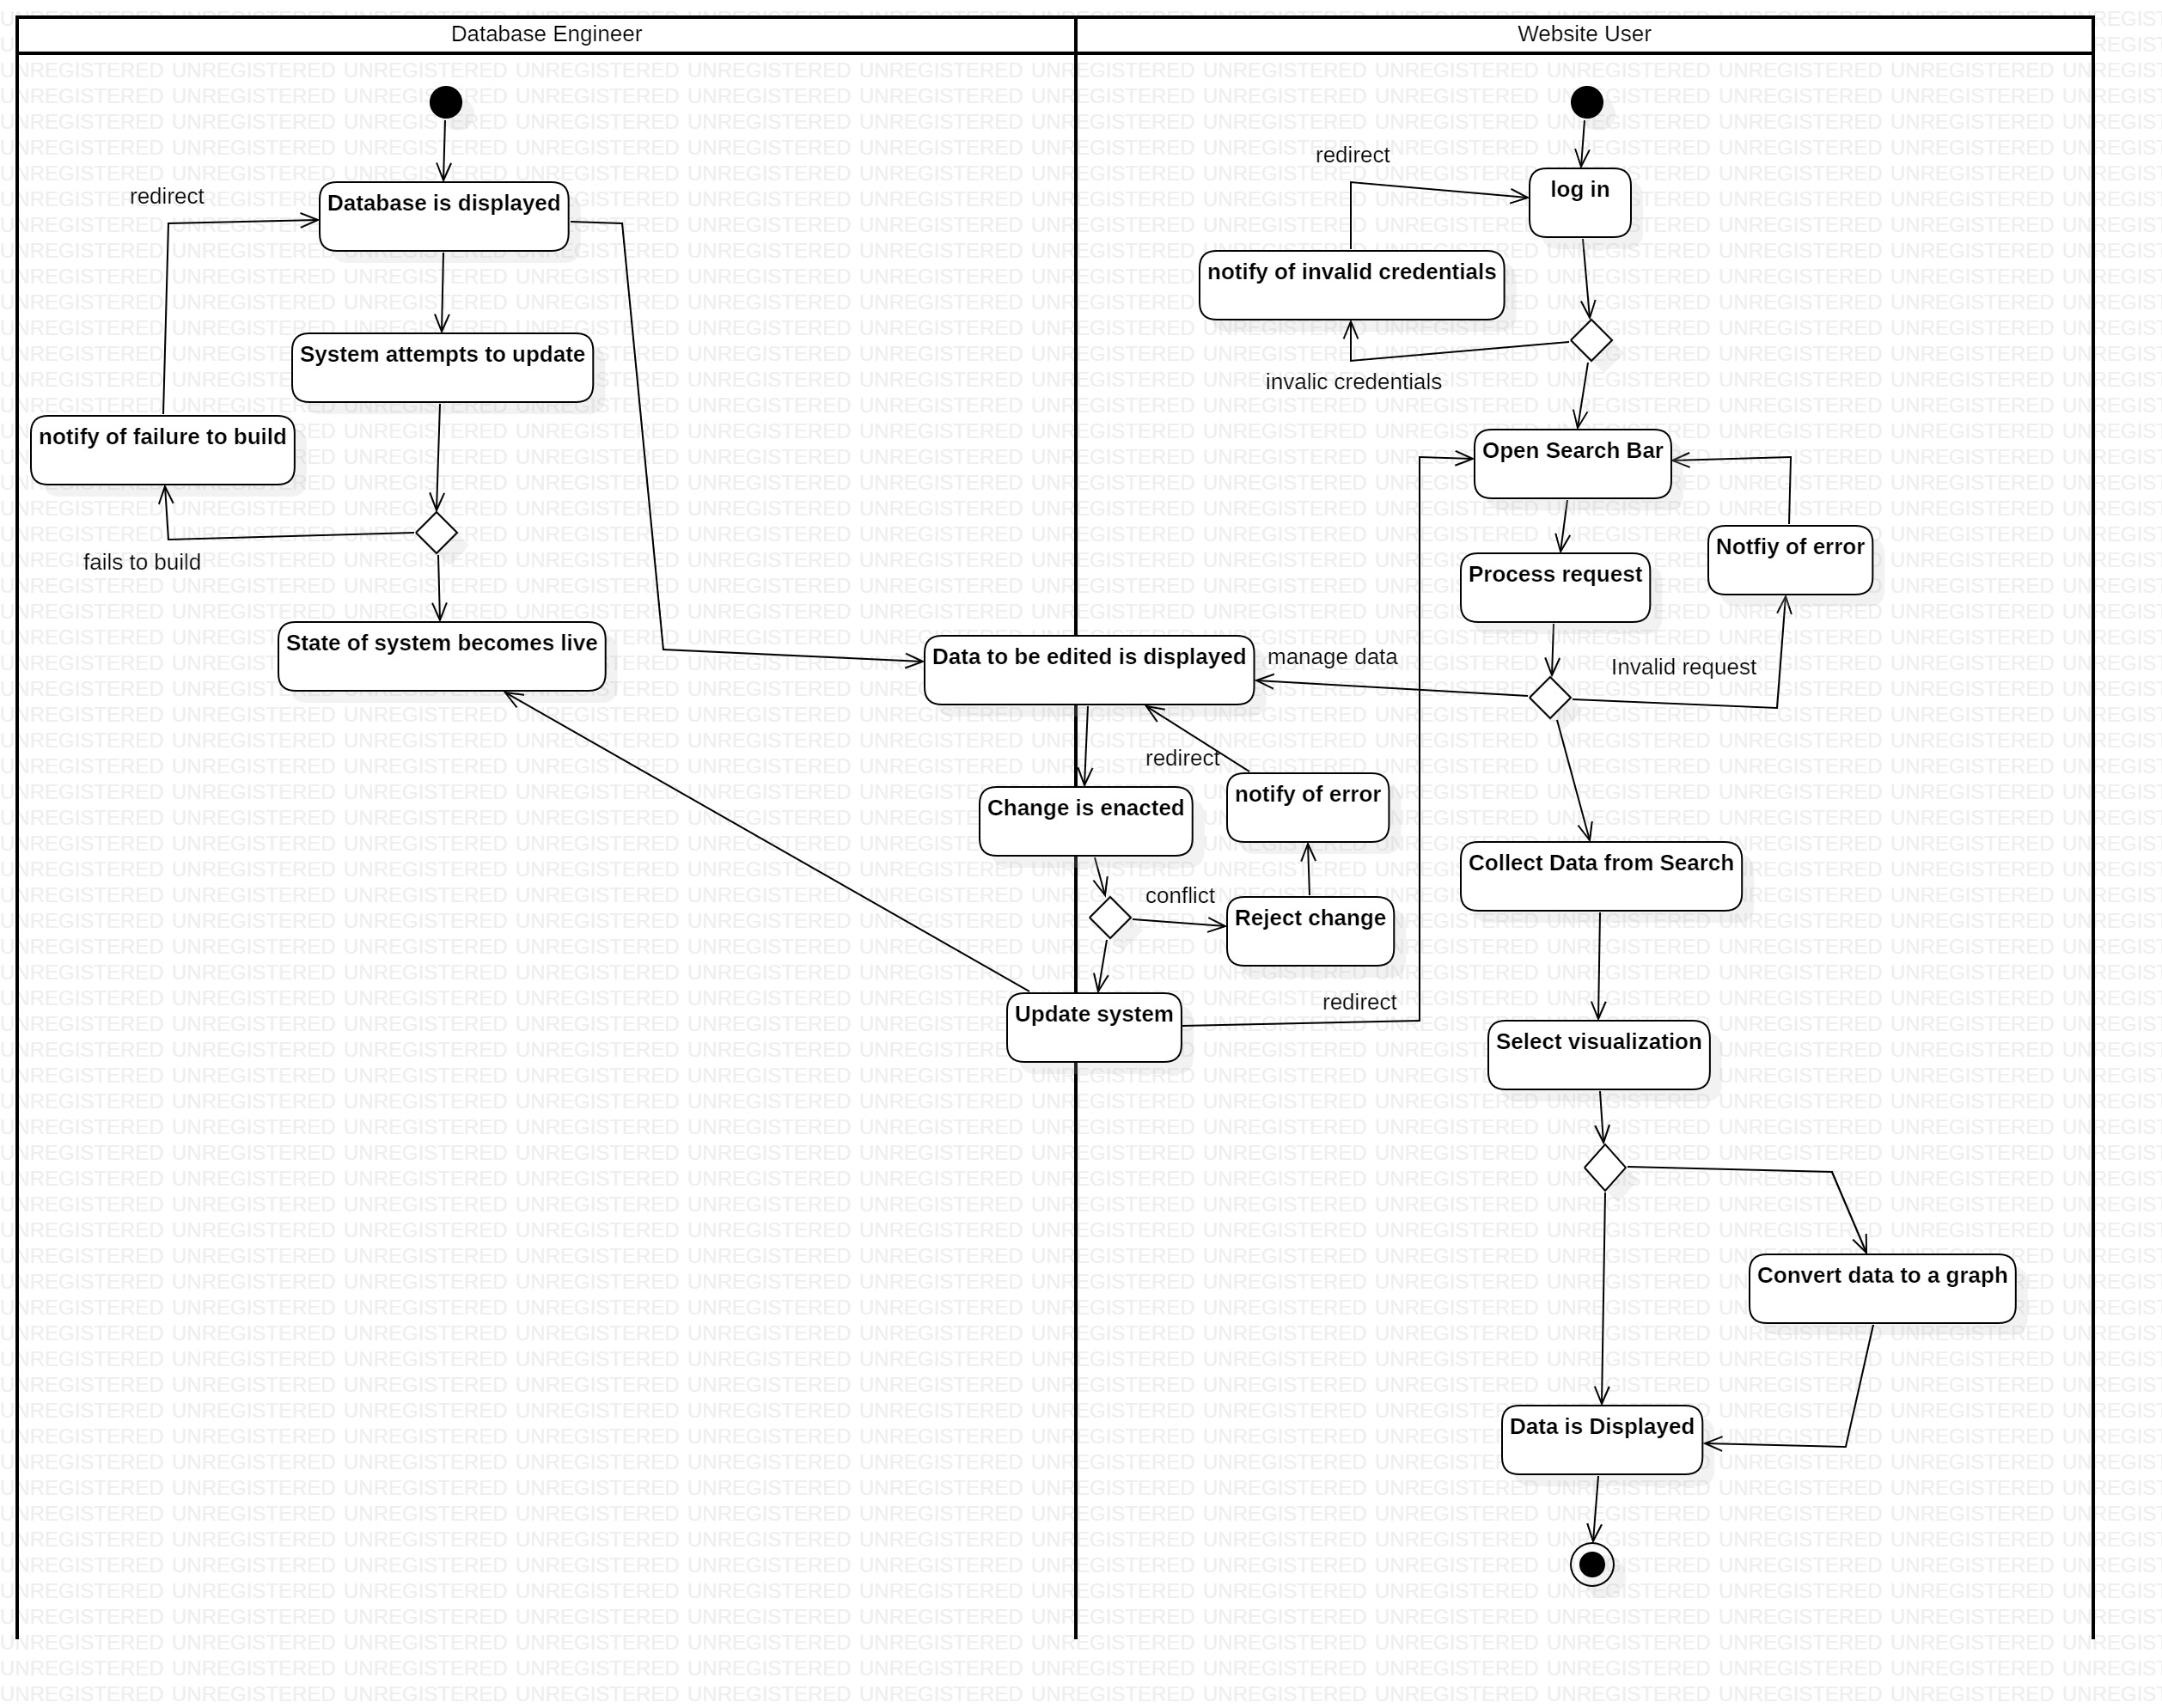
\includegraphics[width=.95\textwidth]{./Activity Diagram/Activitydiagramredo}\\
	\caption{Activity Diagram for the Cold-Cases Database system.}
	\label{fig:activity_diagram}
\end{figure}

\end{document}
